\section{Εισαγωγή στην Επιστήμη της Σύγχρονης Μηχανικής Μάθησης}
\label{sec:theory_ml}

Η εισαγωγή του κλάδου της μηχανικής μάθησης στην επιστήμη των υπολογιστών,
επέτρεψε στους υπολογιστές να μπορούν να αντιμετωπίσουν προβλήματα που εμπλέκουν
την αντίληψη για τον πραγματικό κόσμο και να παίρνουν υποκειμενικές αποφάσεις.

Οι αλγόριθμοι ML, επιτρέπουν σε συστήματα AI
να προσαρμόζονται εύκολα σε καινούργια έργα, με ελάχιστη επέμβαση από τον άνθρωπο.
Για παράδειγμα, ένα Νευρωνικό Δίκτυο που έχει εκπαιδευτεί να αναγνωρίζει γάτες σε εικόνες,
δεν απαιτεί να σχεδιαστεί και να εκπαιδευτεί από το μηδέν για να έχει την ικανότητα
να αναγνωρίζει και σκύλους.

\begin{figure}[!ht]
  \centering
  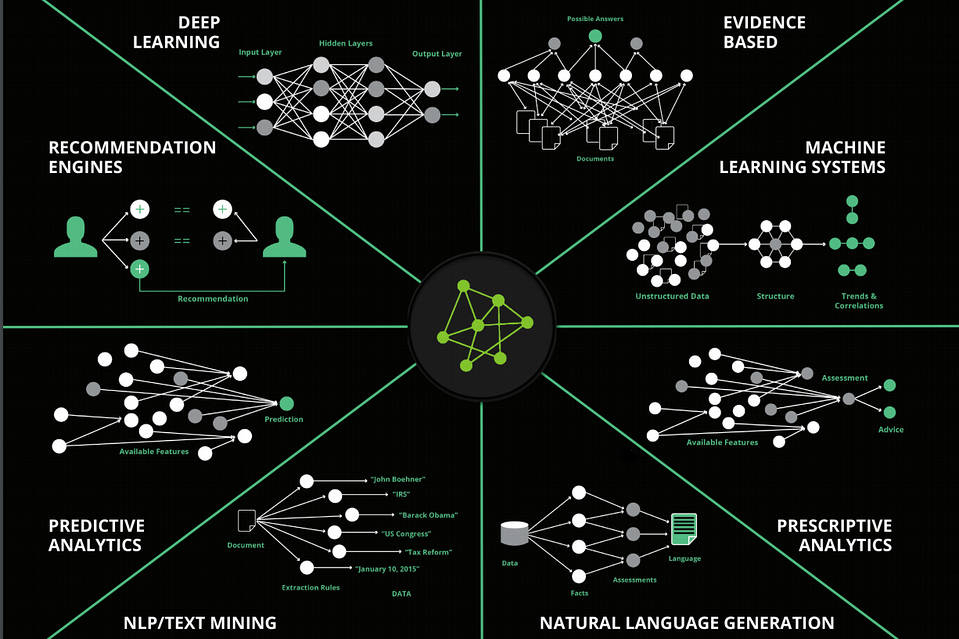
\includegraphics[width=1\textwidth]{./images/chapter3/AI_1.jpg}
  \caption[Κλάδοι και εφαρμογές της επιστήμης της Τεχνητής Νοημοσύνης]{Κλάδοι και εφαρμογές της επιστήμης της Τεχνητής Νοημοσύνης}
  \label{fig:ai_1}
\end{figure}

Πολλά προβλήματα, ενώ μέχρι και πριν μία μερικά χρόνια λύνονταν με
"χειρόγραφη", προγραμματισμένη από τον άνθρωπο γνώση, σήμερα χρησιμοποιούνται
αλγόριθμοι ML για την επίλυσή τους (\autoref{fig:ai_1}). Πιο κάτω παρατίθενται μερικά
παραδείγματα:
\begin{itemize}
  \item{Αναγνώριση ομιλίας - Speech Recognition}
  \item{Μηχανική όραση - Computer Vision}
  \begin{itemize}
    \item{Αναγνώριση αντικειμένων σε εικόνες - Object Recognition}
    \item{Αναγνώριση και εντοπισμός της θέσης αντικειμένων σε εικόνες - Object Detection}
  \end{itemize}
  \item{Αναγνώριση ηλεκτρονικών επιθέσεων στο διαδίκτυο - Cyberattack detection}
  \item{Επεξεργασία φυσικής γλώσσας - Natural Language Processing}
  \begin{itemize}
    \item{Κατανόηση της φυσικής γλώσσας του ανθρώπου - Natural Language Understanding}
    \item{Μοντελοποίηση και χρήση της φυσικής γλώσσας του ανθρώπου από μηχανές - Natural Language Generation}
  \end{itemize}
  \item{Μηχανές αναζήτησης}
  \item{Αναπαράσταση γνώσης - Knowledge Representation}
  \item{Ρομποτική}
\end{itemize}

Τα προβλήματα Μηχανικής Μάθησης χωρίζονται σε τρεις μεγάλες κατηγορίες:
\begin{itemize}
  \item{Υπό επίβλεψη Μάθηση - Supervised Learning:
      Στο υπολογιστικό σύστημα δίνονται παραδείγματα εισόδου και επιθυμητής εξόδου,
      δηλαδή στα δεδομένα έχουν προηγουμένως ανατεθεί ετικέτες(labels),
      και στόχος είναι να μάθει ένα γενικό κανόνα αντιστοίχισης της εισόδου στην επιθυμητή έξοδο.
      Η αναγνώριση αντικειμένων σε εικόνες είναι ένα πρόβλημα που ανήκει σε αυτή την κατηγορία.
    }
  \item{Χωρίς επίβλεψη Μάθηση - Unsupervised Learning:
      Τα δεδομένα δεν έχουν ετικέτες (labels), αφήνοντας έτσι τον αλγόριθμο ML να βρει
      από μόνος του δομές στα δεδομένα εισόδου.
    }
  \item{Εκμάθηση δια ανταμοιβής - Reinforcement Learning:
      Ο πράκτορας αλληλεπιδρά με ένα δυναμικό περιβάλλον στο οποίο πρέπει να
      εκτελέσει ένα συγκεκριμένο στόχο, χωρίς την ύπαρξη ενός "δασκάλου" που να
      ορίζει ρητά αν έχει φθάσει κοντά στον στόχο. Ένα παράδειγμα εφαρμογής
      είναι η αυτόματη πλοήγηση ενός οχήματος.
    }
\end{itemize}
Επιπλέον, κάποια προβλήματα είναι υβριδικά, δηλαδή συνδυασμός των πιο πάνω.
Στο \autoref{fig:ml_venn_diagram} απεικονίζεται το διάγραμμα Venn των διαφόρων κατηγοριών
προβλημάτων ML.
\begin{figure}[!ht]
  \centering
  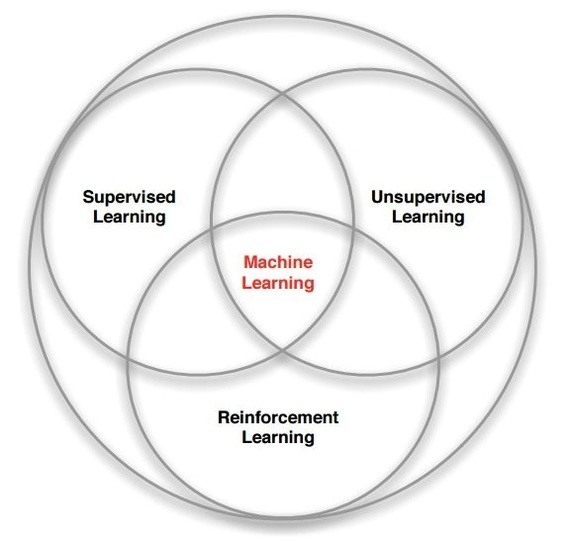
\includegraphics[width=0.7\textwidth]{./images/chapter3/ml_venn_diagram.jpg}
  \caption[Διάγραμμα Venn των διαφόρων κατηγοριών μηχανικής μάθησης]{Διάγραμμα Venn των διαφόρων κατηγοριών μηχανικής μάθησης}
  \label{fig:ml_venn_diagram}
\end{figure}

Περαιτέρω, οι Supervised Learning αλγόριθμοι χωρίζονται σε 2 κατηγορίες, ανάλογα
με την επιθυμητή μορφή της εξόδου του αλγόριθμου ML:
\begin{itemize}
  \item{Ταξινόμησης - Classification: Όταν η έξοδος παίρνει διακριτές τιμές (discrete).}
  \item{Regression: Όταν η έξοδος παίρνει συνεχείς τιμές.}
\end{itemize}

Γενικότερα, οι αλγόριθμοι ML ομαδοποιούνται και ανάλογα με την ομοιότητα τους
σε σχέση με με την λειτουργία που εκτελούν. Πιο κάτω αναφέρονται οι πιο δημοφιλείς
αλγόριθμοι ML, ομαδοποιημένοι με βάση την λειτουργία τους
\\

\begin{minipage}{0.5\textwidth}

  \textbf{\large Regression}

  Ασχολείται με τη μοντελοποίηση της σχέσης μεταξύ των μεταβλητών που επαναληπτικά ανανεώνονται
  χρησιμοποιώντας ένα μέτρο σφάλματος για τις προβλέψεις που γίνονται από το μοντέλο
  \begin{itemize}
    \setlength\itemsep{0em}
    \item{Ordinary Least Squares Regression (OLSR)}
    \item{Linear Regression}
    \item{Logistic Regression}
    \item{Stepwise Regression}
    \item{Multivariate Adaptive Regression Splines (MARS)}
    \item{Locally Estimated Scatterplot Smoothing (LOESS)}
  \end{itemize}
\end{minipage}
\begin{minipage}{0.5\textwidth}
  \begin{center}
    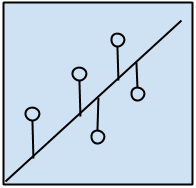
\includegraphics[width=0.6\textwidth]{./images/chapter3/regression_algorithms.png}
  \end{center}
\end{minipage}

\begin{minipage}{0.5\textwidth}

  \textbf{\large Instance-based}

  Αυτές οι μέθοδοι δημιουργούν μία βάση δεδομένων με
  παραδείγματα δεδομένων και συγκρίνουν τα νέα δεδομένα με αυτά που έχουν
  καταχωρηθεί στην βάση δεδομένων χρησιμοποιώντας ένα μέτρο ομοιότητας,
  για την εύρεση της καλύτερης αντιστοιχίας, πιθανοτικά.
  \begin{itemize}
    \setlength\itemsep{0em}
    \item{k-Nearest Neighbour (kNN)}
    \item{Learning Vector Quantization (LVQ)}
    \item{Self-Organizing Map (SOM)}
    \item{Locally Weighted Learning (LWL)}
  \end{itemize}
\end{minipage}
\begin{minipage}{0.5\textwidth}
  \begin{center}
    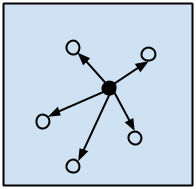
\includegraphics[width=0.6\textwidth]{./images/chapter3/instance_based_algorithms.png}
  \end{center}
\end{minipage}

\begin{minipage}{0.5\textwidth}  %% Minipage

  \textbf{\large Regularization}

  Χρησιμοποιούνται σαν επεκτάσεις άλλων μεθόδων και
  "τιμωρούν" μοντέλα, βασισμένα στην πολυπλοκότητα τους, ευνοώντας έτσι
  απλούστερα μοντέλα τα οποίο είναι παράλληλα καλύτερα στην γενίκευση της
  επίλυσης του εκάστοτε προβλήματος.
  \begin{itemize}
    \setlength\itemsep{0em}
    \item{Ridge Regression}
    \item{Least Absolute Shrinkage and Selection Operator (LASSO)}
    \item{Least-Angle Regression (LARS)}
    \item{Elastic Net}
  \end{itemize}
\end{minipage}
\begin{minipage}{0.5\textwidth}
  \begin{center}
    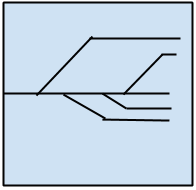
\includegraphics[width=0.6\textwidth]{./images/chapter3/regularization_algorithms.png}
  \end{center}
\end{minipage}

\begin{minipage}{0.5\textwidth}

  \textbf{\large Dimensionality Reduction}

  Χρησιμοποιούνται για την αφαίρεση σχεδόν ασήμαντης πληροφορίας
  από τα δεδομένα. Πολλές από τις μεθόδους αυτές χρησιμοποιούνται σαν επεκτάσεις σε μοντέλα επίλυσης
  προβλημάτων regression και classification

  \begin{itemize}
    \setlength\itemsep{0em}
    \item{Principal Component Analysis (PCA)}
    \item{Discriminant Analysis: Linear (LDA), Mixture (MDA), Quadratic (QDA), Flexible (FDA)}
    \item{Principal Component Regression (PCR)}
    \item{Multidimensional Scaling (MDS)}
  \end{itemize}
\end{minipage}
\begin{minipage}{0.5\textwidth}
  \begin{center}
    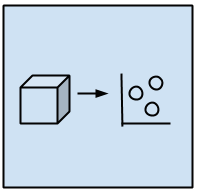
\includegraphics[width=0.6\textwidth]{./images/chapter3/dimensional_reduction_algorithms.png}
  \end{center}
\end{minipage}

\begin{minipage}{0.5\textwidth}

  \textbf{\large Decision Trees}

  Χρησιμοποιούνται για την κατασκευή μοντέλων
  λήψης αποφάσεων, τα οποία χρησιμοποιούν τις πραγματικές τιμές των
  χαρακτηριστικών των δεδομένων.
  \begin{itemize}
    \setlength\itemsep{0em}
    \item{Classification and Regression Tree (CART)}
    \item{Conditional Decision Trees}
    \item{M5}
  \end{itemize}
\end{minipage}
\begin{minipage}{0.5\textwidth}
  \begin{center}
    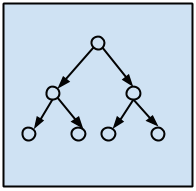
\includegraphics[width=0.6\textwidth]{./images/chapter3/decision_tree_algorithms.png}
  \end{center}
\end{minipage}

\begin{minipage}{0.5\textwidth}

  \textbf{\large Bayesian}

  Εφαρμόζουν το θεώρημα του Bayes για την επίλυση τόσο προβλημάτων regression, αλλά και classification
  \begin{itemize}
    \setlength\itemsep{0em}
    \item{Naive Bayes}
    \item{Gaussian Naive Bayes}
    \item{Bayesian Network (BN)}
    \item{Bayesian Belief Network (BBN)}
  \end{itemize}
\end{minipage}
\begin{minipage}{0.5\textwidth}
  \begin{center}
    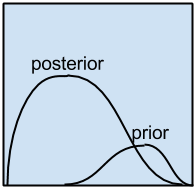
\includegraphics[width=0.6\textwidth]{./images/chapter3/bayesian_algorithms.png}
  \end{center}
\end{minipage}

\begin{minipage}{0.5\textwidth}

  \textbf{\large Clustering}

  Περιγράφουν τις κλάσεις του προβλήματος
  \begin{itemize}
    \setlength\itemsep{0em}
    \item{k-Means}
    \item{k-Medians}
    \item{Expectation Maximisation (EM)}
    \item{Hierarchical Clustering}
  \end{itemize}
\end{minipage}
\begin{minipage}{0.5\textwidth}
  \begin{center}
    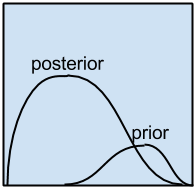
\includegraphics[width=0.6\textwidth]{./images/chapter3/bayesian_algorithms.png}
  \end{center}
\end{minipage}

\begin{minipage}{0.5\textwidth}

  \textbf{\large Artificial Neural Networks (ANN)}

  Μοντέλα εμπνευσμένα από τη δομή ή/και την λειτουργία των βιολογικών νευρωνικών δικτύων.
  Χρησιμοποιούνται στην επίλυση προβλημάτων classification ή/και regression
  \begin{itemize}
    \setlength\itemsep{0em}
    \item{Perceptron}
    \item{Back-Propagation}
    \item{Radial Basis Function Network (RBFN)}
  \end{itemize}
\end{minipage}
\begin{minipage}{0.5\textwidth}
  \begin{center}
    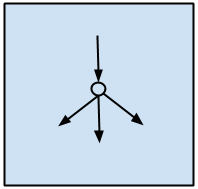
\includegraphics[width=0.6\textwidth]{./images/chapter3/artificial_neural_network_algorithms.png}
  \end{center}
\end{minipage}

\begin{minipage}{0.5\textwidth}

  \textbf{\large Deep Learning (DL)}

  Οι αλγόριθμοι DL είναι η σύγχρονη επέκταση των ANN, τα οποία
  εκμεταλλεύονται την αφθονία υπολογιστικής ισχύς των σύγχρονων υπολογιστικών συστημάτων.
  \begin{itemize}
    \setlength\itemsep{0em}
    \item{Autoncoder}
    \item{Multilayer Perseptron (MLP)}
    \item{Deep Boltzmann Machine (DBM)}
    \item{Deep Belief Networks (DBN)}
    \item{Convolutional Neural Network (CNN)}
    \item{Stacked Auto-Encoders}
    \item{Recurrent Neural Networks (RNN)}
  \end{itemize}%
\end{minipage}
\begin{minipage}{0.5\textwidth}
  \begin{center}
    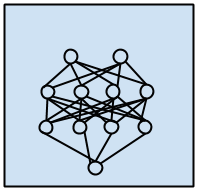
\includegraphics[width=0.6\textwidth]{./images/chapter3/deep_learning_algorithms.png}
  \end{center}
\end{minipage}
\\\\

Η μορφή της αναπαράστασης των δεδομένων αποτελεί σημαντικό παράγοντα στην
απόδοση των αλγορίθμων ML. Μία αναπαράσταση αποτελείται από χαρακτηριστικά (features).
Για παράδειγμα, ένα χρήσιμο χαρακτηριστικό, στην ταυτοποίηση ομιλητή, από δεδομένα ήχου,
είναι η εκτίμηση του μεγέθους της φωνητικής έκτασης του ομιλητή.
Έτσι, πολλά προβλήματα τεχνητής νοημοσύνης, μπορούν να λυθούν
με κατάλληλη σχεδίαση και επιλογή των χαρακτηριστικών, για το συγκεκριμένο
πρόβλημα. Το σύνολο των χαρακτηριστικών αυτών αποτελεί την αναπαράσταση των δεδομένων,
σε ένα πιο υψηλό και αφαιρετικό επίπεδο αντίληψης για τους υπολογιστές, η οποία
στην συνέχεια δίνεται σαν είσοδος σε έναν απλό ML αλγόριθμο, ο οποίος έχει
μάθει να αντιστοιχεί την αναπαράσταση των δεδομένων στην επιθυμητή έξοδο.
\begin{figure}[!h]
  \centering
  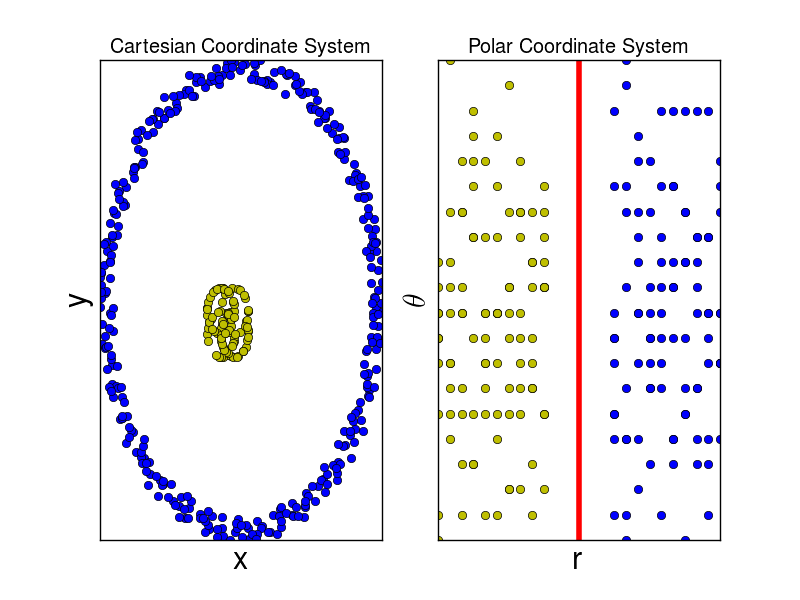
\includegraphics[width=0.7\textwidth]{./images/chapter3/representation_dependency.png}
  \caption[Παράδειγμα διαφορετικών αναπαραστάσεων των δεδομένων]{Παράδειγμα διαφορετικών αναπαραστάσεων των δεδομένων}
  \label{fig:representation_dependency}
\end{figure}

Ένα απλό και κατανοητό παράδειγμα το οποίο δείχνει την εξάρτηση της επίδοσης των
αλγορίθμων ML από την μορφή της αναπαράστασης που του δίνεται, φαίνεται στο
\autoref{fig:representation_dependency}. Έστω ότι θέλουμε να
διαχωρίσουμε τα δεδομένα μας σε δύο κλάσεις, χαράζοντας μία ευθεία
μεταξύ τους. Αν αναπαραστήσουμε τα δεδομένα στο Καρτεσιανό σύστημα συντεταγμένων (αριστερό διάγραμμα),
τότε η επίλυση του προβλήματος είναι αδύνατη αφού δεν υπάρχει καμία ευθεία
που να διαχωρίζει τις δύο κλάσεις. Ωστόσο, αν αναπαραστήσουμε τα δεδομένα
στο Πολικό σύστημα συντεταγμένων (δεξί διάγραμμα), τότε το πρόβλημα λύνεται
εύκολα, χαράζοντας μία κάθετη ευθεία, με $r  = a, a \in [r1, r2]$.

Σε πληθώρα προβλημάτων τεχνητής νοημοσύνης, η επιλογή κατάλληλων χαρακτηριστικών
είναι δύσκολο και χρονοβόρο έργο. Έστω για παράδειγμα ότι θέλουμε να αναγνωρίσουμε
πρόσωπα σε εικόνες. Ένα χαρακτηριστικό θα μπορούσε να είναι τα μάτια. Δυστυχώς όμως,
η αναγνώριση ματιών είναι και αυτό ένα δύσκολο πρόβλημα, αφού δεν μπορεί να
περιγραφεί πάντα επακριβώς έχοντας σαν δεδομένα τις τιμές των pixel της εικόνας.
Η γεωμετρική, για παράδειγμα, μορφή των ματιών σε μία εικόνα λήψης εξαρτάται από την
γωνία λήψης της εικόνας, τον φωτισμό, τις ανακλάσεις του φωτισμού,
την απόσταση από την οποία γίνεται η λήψη, την ανάλυση της κάμερας, κτλ.

Το πρόβλημα αυτό, της επιλογής κατάλληλης αναπαράστασης, μπορεί να λυθεί
χρησιμοποιώντας τεχνικές μηχανικής μάθησης για την εκμάθηση της ίδιας
της αναπαράστασης. Αυτή η προσέγγιση είναι γνωστή ως
\emph{Εκμάθηση Αναπαραστάσεων (Representation Learning)}. Οι αλγόριθμοι
εκμάθησης αναπαραστάσεων είναι ικανοί να "μάθουν" ένα καλό σετ χαρακτηριστικών (features).
\begin{figure}[!ht]
  \centering
  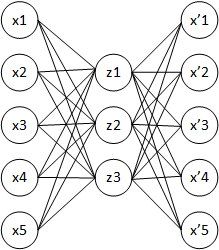
\includegraphics[width=0.3\textwidth]{./images/chapter3/autoencoder.png}
  \caption[Απλό μοντέλο Autoncoder με ένα κρυφό επίπεδο]{Απλό μοντέλο Autoncoder με ένα κρυφό επίπεδο.}
  \label{fig:autoencoder}
\end{figure}
Ένα απλό παράδειγμα αλγορίθμου εκμάθησης αναπαραστάσεων είναι αυτό του
Autoencoder \cite{baldi2012autoencoders} που φαίνεται στο (\autoref{fig:autoencoder}).
Ο Autoencoder, στην πιο απλή του μορφή, είναι ο συνδυασμός ενός κωδικοποιητή (encoder) ο οποίος μετατρέπει
τα δεδομένα εισόδου σε μία διαφορετική αναπαράσταση, και ενός αποκωδικοποιητή
ο οποίος επαναφέρει την αναπαράσταση αυτή στην αρχική μορφή της αναπαράστασης των
δεδομένων εισόδου. Οι Autoencoders ανήκουν στην κατηγορία των Νευρωνικών
Δικτύων και είναι Unsupervised ML αλγόριθμοι.
\begin{figure}[!ht]
  \centering
  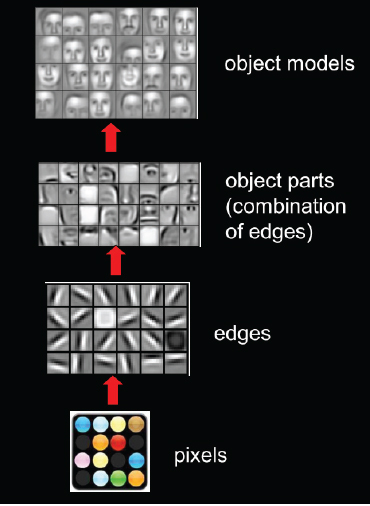
\includegraphics[width=0.5\textwidth]{./images/chapter3/cnn_deeper.jpg}
  \caption[Παράδειγμα απεικόνισης των φίλτρων ενός μοντέλου CNN για αναγνώριση προσώπου]{Παράδειγμα απεικόνισης των φίλτρων ενός μοντέλου CNN για αναγνώριση προσώπου}
  \label{fig:cnn_filter_visualization}
\end{figure}
Ένα συχνά εμφανιζόμενο πρόβλημα σε εφαρμογές τεχνητής νοημοσύνης είναι
η εύρεση και εξαγωγή χαρακτηριστικών \emph{υψηλού επιπεδου} από τα
δεδομένα. Τα μοντέλα \emph{Βαθιάς Μηχανικής Μάθησης} δίνουν λύσεις
σε αυτό το πρόβλημα εμκάθησης αναπαραστάσεων με την εισαγωγή αναπαραστάσεων
οι οποίες εκφράζονται με βάση άλλες, απλούστερες αναπαραστάσεις. Αυτή η
προσέγγιση δίνει την δυνατότητα στους υπολογιστές να κατασκευάζουν σύνθετες
έννοιες χρησιμοποιώντας πιο απλές έννοιες. Για παράδειγμα, η αναγνώριση αντικειμένων
μπορεί να εκφραστεί με έννοιες όπως το γεωμετρικό σχήμα των αντικειμένων,
το οποίο με την σειρά του ορίζεται από γωνίες και περιγράμματα. Επίσης,
οι γωνίες και τα περιγράμματα ορίζονται από ακμές. Στο \autoref{fig:cnn_filter_visualization},
παρουσιάζονται τα φίλτρα που έμαθε ένα μοντέλο CNN για αναγνώριση προσώπων σε εικόνες.
Το συγκεκριμένο μοντέλο CNN έχει 3 κρυφά επίπεδα (hidden layers); το πρώτο κρυφό
επίπεδο εξάγει από τα δεδομένα εισόδου (τιμές των πίξελ) πληροφορία σχετικά με
τις ακμές, το δεύτερο, έχοντας σαν είσοδο την πληροφορία παρουσίας ακμών, εξάγει πληροφορία
σχετικά με τις γωνίες και τα περιγράμματα, και το τρίτο παίρνει σαν είσοδο
την πληροφορία αυτή και κατασκευάζει μοντέλα αντικειμένων, δηλαδή εξάγει πληροφορία
σχετικά με το γεωμετρικό σχήμα των αντικειμένων.

Συνοψίζοντας, η βαθιά μηχανική μάθηση, είναι μία προσέγγιση της σύγχρονης
τεχνητής νοημοσύνης. Πιο συγκεκριμένα, είναι ένα είδος μηχανικής μάθησης, η
οποία προσδίδει σε υπολογιστικά συστήματα ευφυΐα, δηλαδή την ικανότητα
εξέλιξης με την χρήση εμπειρίας και δεδομένων. Σύμφωνα με τους
\emph{Ian Goodfellow, Yoshua Bengio και Aaron Courville}, η μηχανική μάθηση είναι η
μόνη βιώσιμη προσέγγιση στην κατασκευή συστημάτων AI τα οποία μπορούν να
αντεπεξέλθουν σε πολύπλοκα περιβάλλοντα και προβλήματα \cite{Goodfellow-et-al-2016-Book}.
Η βαθιά μηχανική μάθηση καταφέρνει να μαθαίνει να αναπαριστά τον κόσμο ως μία ένθετη
ιεραρχία εννοιών όπου η κάθε έννοια ορίζεται σε σχέση με άλλες πιο απλές έννοιες,
και πιο αφηρημένες μορφές αναπαραστάσεων σε σχέση με λιγότερο αφηρημένες.
Από το διάγραμμα Venn που βλέπουμε στο \autoref{fig:ai_venn_diagram} παρατηρούμε
ότι η βαθιά μηχανική μάθηση ανήκει στην κατηγορία της εκμάθησης αναπαραστάσεων,
η οποία με την σειρά της είναι ένα είδος μηχανικής μάθησης που χρησιμοποιείται
για την κατασκευή νοούμενων συστημάτων.

\begin{figure}[!ht]
  \centering
  \includegraphics[width=0.9\textwidth]{./images/chapter3/ai_venn_diagram.png}
  \caption[Παράδειγμα απεικόνισης των φίλτρων ενός μοντέλου CNN για αναγνώριση προσώπου]{Παράδειγμα απεικόνισης των φίλτρων ενός μοντέλου CNN για αναγνώριση προσώπου}
  \label{fig:ai_venn_diagram}
\end{figure}
